\begin{frame}{Preface: Decision Trees}
    \begin{itemize}
        \item Decision trees are part of ML since 1980s
        \begin{itemize}
            \item Introduced by Leo Breiman in 1984
            \item Notable algorithms: ID3, C4.5
        \end{itemize}
        \item More recent innovations include:
        \begin{itemize}
            \item Boosted decision trees (gradient boosted DT)
            \item Random forest
        \end{itemize}
        \item Even though DTs are old, hand-engineered and heuristic, they are a method of choice for tabular data and for Kaggle competitions. 🙂
    \end{itemize}
\end{frame}


\begin{frame}{Decision Tree Learning}
    \begin{itemize}
        \item Given one attribute (e.g., lifespan), try to predict the value of new people’s lifespans by a subset of the other available attributes

        \item Input attributes:
        \begin{itemize}
            \item d features/attributes: $x^{(1)}, x^{(2)}, \ldots, x^{(d)}$
            \item Each $x^{(j)}$ has domain $O_j$
            \begin{itemize}
                \item Categorical: $O_j = \{male, female, nonbinary\}$
                \item Numerical: $H_j = (1, 200)$
            \end{itemize}
            \item $Y$ is output variable with domain $O_Y$:
            \begin{itemize}
                \item Categorical: Classification e.g. $Y$ = eye color
                \item Numerical: Regression e.g. $Y$ = lifespan
            \end{itemize}
        \end{itemize}

        \item Data D:
        \begin{itemize}
            \item $n$ examples $(x_i, y_i)$ where $x_i$ is a $d$-dim feature vector, $y_i \in O_Y$ is output variable
        \end{itemize}

        \item Task:
        \begin{itemize}
            \item Given an input data vector $x$ predict output label $y$
        \end{itemize}
    \end{itemize}
\end{frame}


\begin{frame}{Decision Trees}
    \begin{columns}
        \begin{column}{0.5\textwidth}
            \begin{itemize}
                \item A Decision Tree is a tree-structured plan of a set of attributes to test in order to predict the output
            \end{itemize}
        \end{column}
        \begin{column}{0.5\textwidth}
            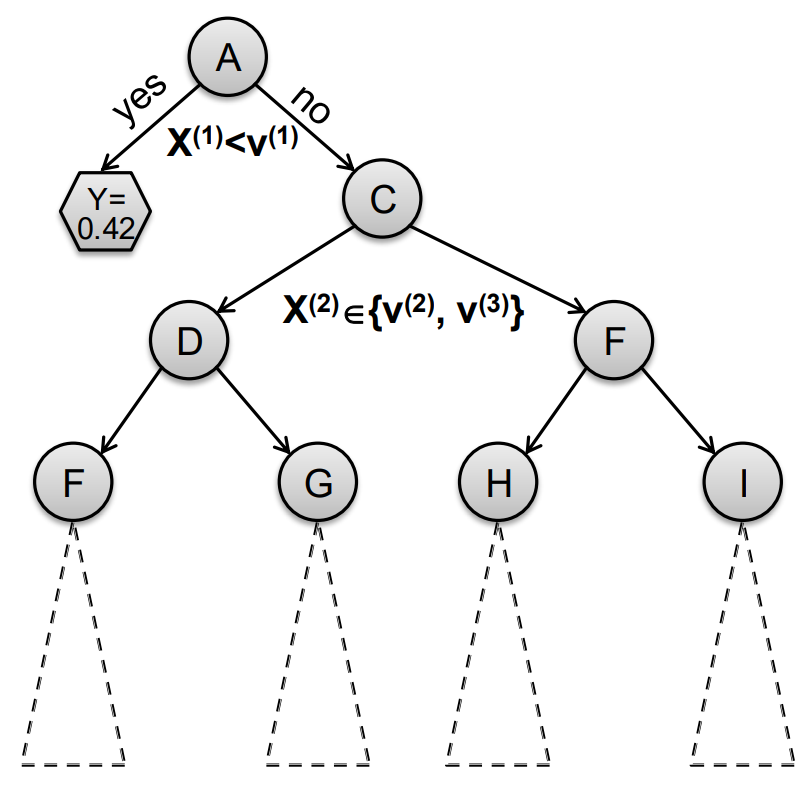
\includegraphics[width=\linewidth]{images/decision-trees/decision-trees-3.png}
        \end{column}
    \end{columns}
\end{frame}


\begin{frame}{Decision Trees}
    \begin{columns}
        \begin{column}{0.5\textwidth}
            \begin{itemize}
                \item \textbf{Decision trees:}
                \begin{itemize}
                    \item Split the data at each internal node
                    \item Each leaf node makes a prediction
                \end{itemize}
                \item \textbf{Lecture today:}
                \begin{itemize}
                    \item Binary splits: $x^{(j)} < v$
                    \item Numerical attributes
                    \item Regression
                \end{itemize}
            \end{itemize}
        \end{column}
        \begin{column}{0.5\textwidth}
            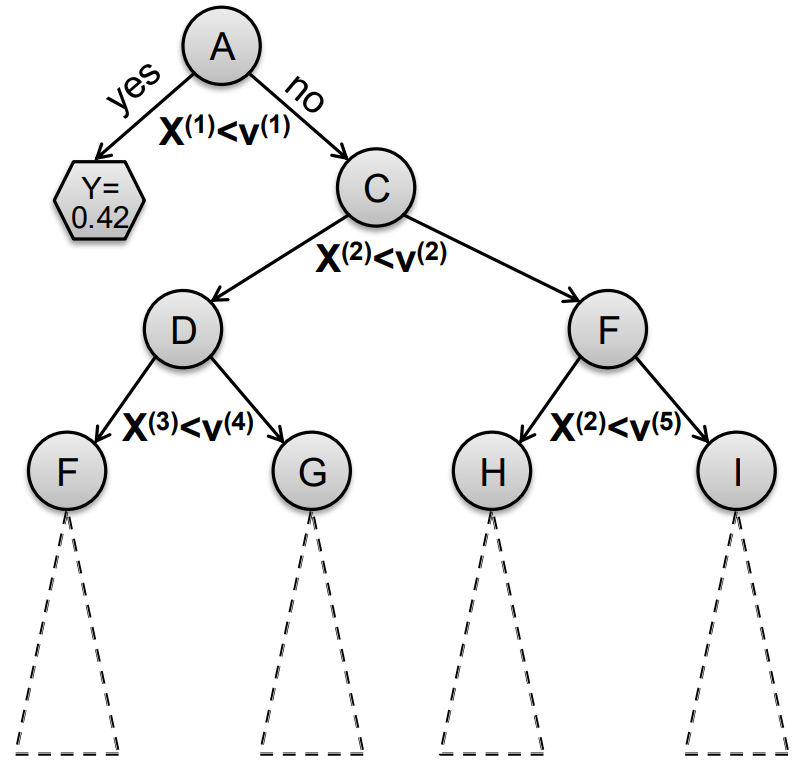
\includegraphics[width=\linewidth]{images/decision-trees/decision-trees-4.png}
        \end{column}
    \end{columns}
\end{frame}


\begin{frame}{How to make predictions?}
    \begin{columns}
        \begin{column}{0.5\textwidth}
            \begin{itemize}
                \item Input: Example $x_i$
                \item Output: Predicted $\hat{y}_i$
                \item “Drop” $x_i$ down the tree until it hits a leaf node
                \item Predict the value stored in the leaf that $x_i$ hits
            \end{itemize}
        \end{column}
        \begin{column}{0.5\textwidth}
            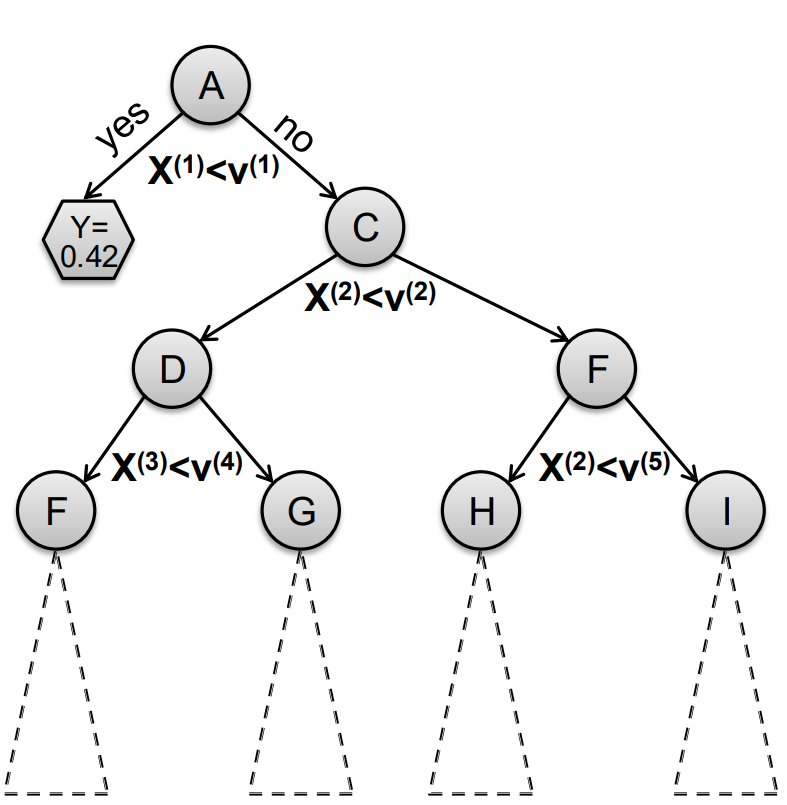
\includegraphics[width=\linewidth]{images/decision-trees/decision-trees-5.png}
        \end{column}
    \end{columns}
\end{frame}

\begin{frame}{Decision Trees: feature space}
    \begin{itemize}
        \item \textbf{Alternative view:}
        \end{itemize}
        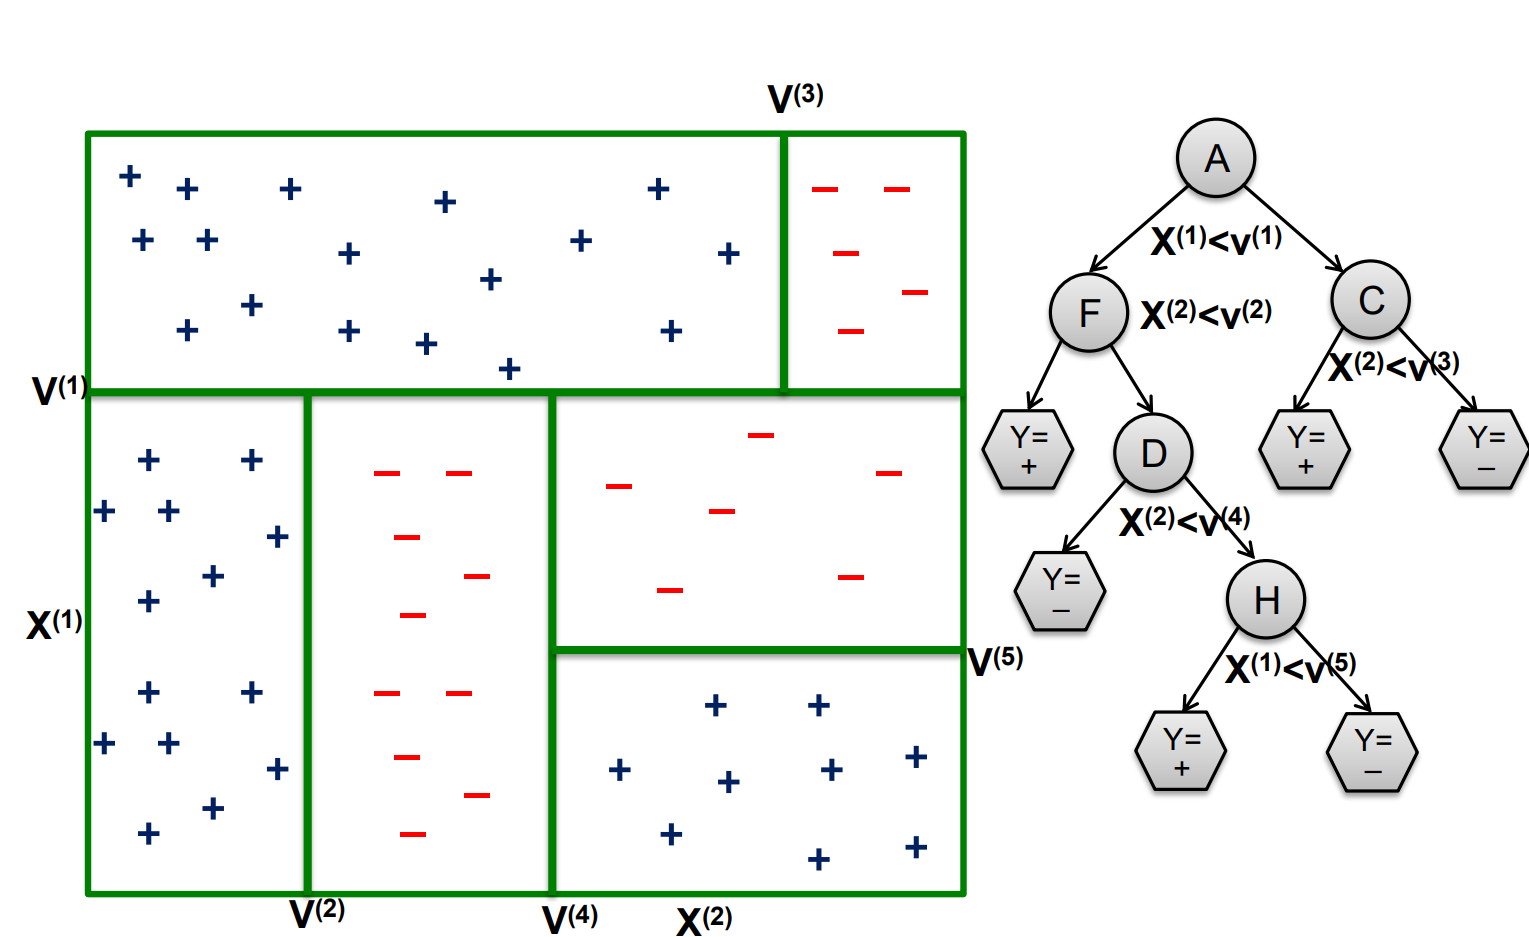
\includegraphics[width=\linewidth]{images/decision-trees/decision-trees-6.png}
\end{frame}


\begin{frame}{Training dataset $D^*$, $|D^*| = 100$ examples}
    \begin{itemize}
        \item Training dataset $D^*$, $|D^*| = 100$ examples
    \end{itemize}

    \begin{center}
        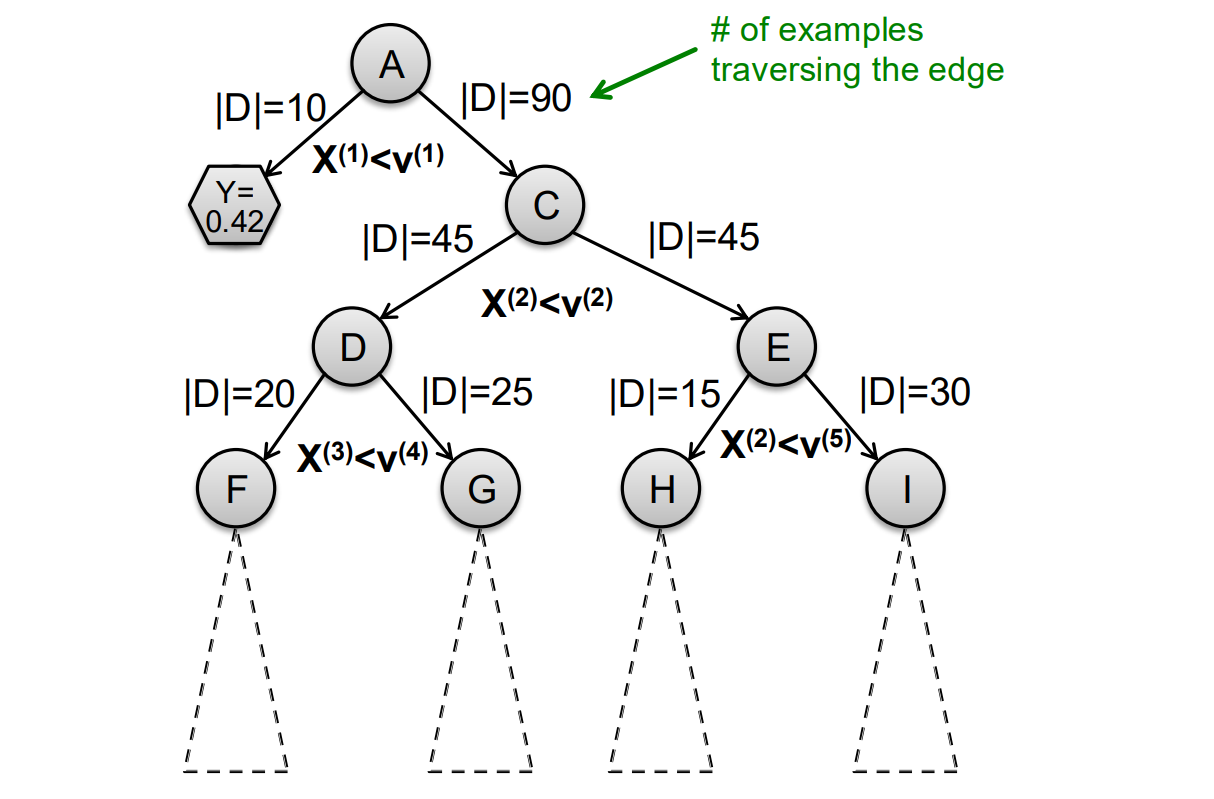
\includegraphics[width=0.8\linewidth]{images/decision-trees/decision-trees-7.png}
    \end{center}
\end{frame}


\begin{frame}{How to construct a tree?}
    \begin{columns}
        \begin{column}{0.55\textwidth}
            \begin{itemize}
                \item Imagine we are currently at some node $G$
                \begin{itemize}
                    \item Let $D_G$ be the data that reaches $G$
                \end{itemize}
                \item There is a decision we have to make: Do we continue building the tree?
                \begin{itemize}
                    \item If yes, which variable and which value do we use for a split?
                    \begin{itemize}
                        \item Continue building the tree recursively
                    \end{itemize}
                    \item If not, how do we make a prediction?
                    \begin{itemize}
                        \item We need to build a “predictor node”
                    \end{itemize}
                \end{itemize}
            \end{itemize}
        \end{column}
        \begin{column}{0.45\textwidth}
            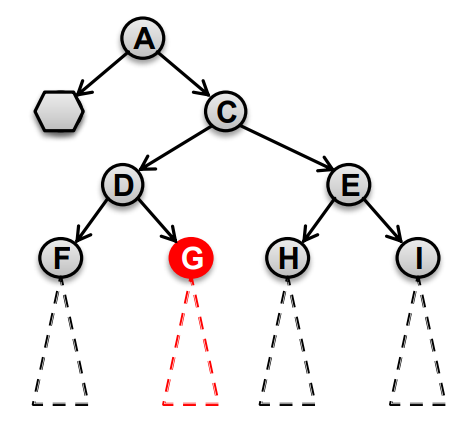
\includegraphics[width=\linewidth]{images/decision-trees/decision-trees-8.png}
        \end{column}
    \end{columns}
\end{frame}


